\documentclass[aspectratio=43]{beamer}
\usepackage{ragged2e}
\usepackage{multirow}
\usepackage{alltt}

\usetheme{CSCS}


\newcommand{\SummerSchoolYear}{2016}
\newcommand{\SummerSchoolDate}{July 20 -- 21}
\newcommand{\SummerSchoolAuthor}{Maxime Martinasso}

\newcommand{\footlinetext}{Summer School \SummerSchoolYear{} -- MPI}

\author{\SummerSchoolAuthor, CSCS}
\title{Message Passing Interface (MPI)}
\subtitle{Summer School \SummerSchoolYear{}  -- Effective High Performance Computing}
\date{\SummerSchoolDate, \SummerSchoolYear}

\title{MPI RMA -  One sided communication}

% Select the image for the title page
%\newcommand{\picturetitle}{cscs_images/image3.pdf}
\newcommand{\picturetitle}{cscs_images/image5.pdf}
%\newcommand{\picturetitle}{cscs_images/image6.pdf}

\begin{document}

% TITLE SLIDE
\cscstitle

\begin{frame}{Course Objectives}
\begin{itemize}
\item One sided MPI communication
\end{itemize}
\end{frame}

% CHAPTER SLIDE
\cscschapter{One sided communication}

\begin{frame}[fragile]{Main concepts}
\begin{itemize}
    \item A memory region is exposed by all ranks (window)
    \item Each rank can read or write in a region
    \item Transfers and synchronisation are decoupled
\end{itemize}
\end{frame}

\begin{frame}[fragile]{2-sided vs 1-sided}
    \begin{center}
        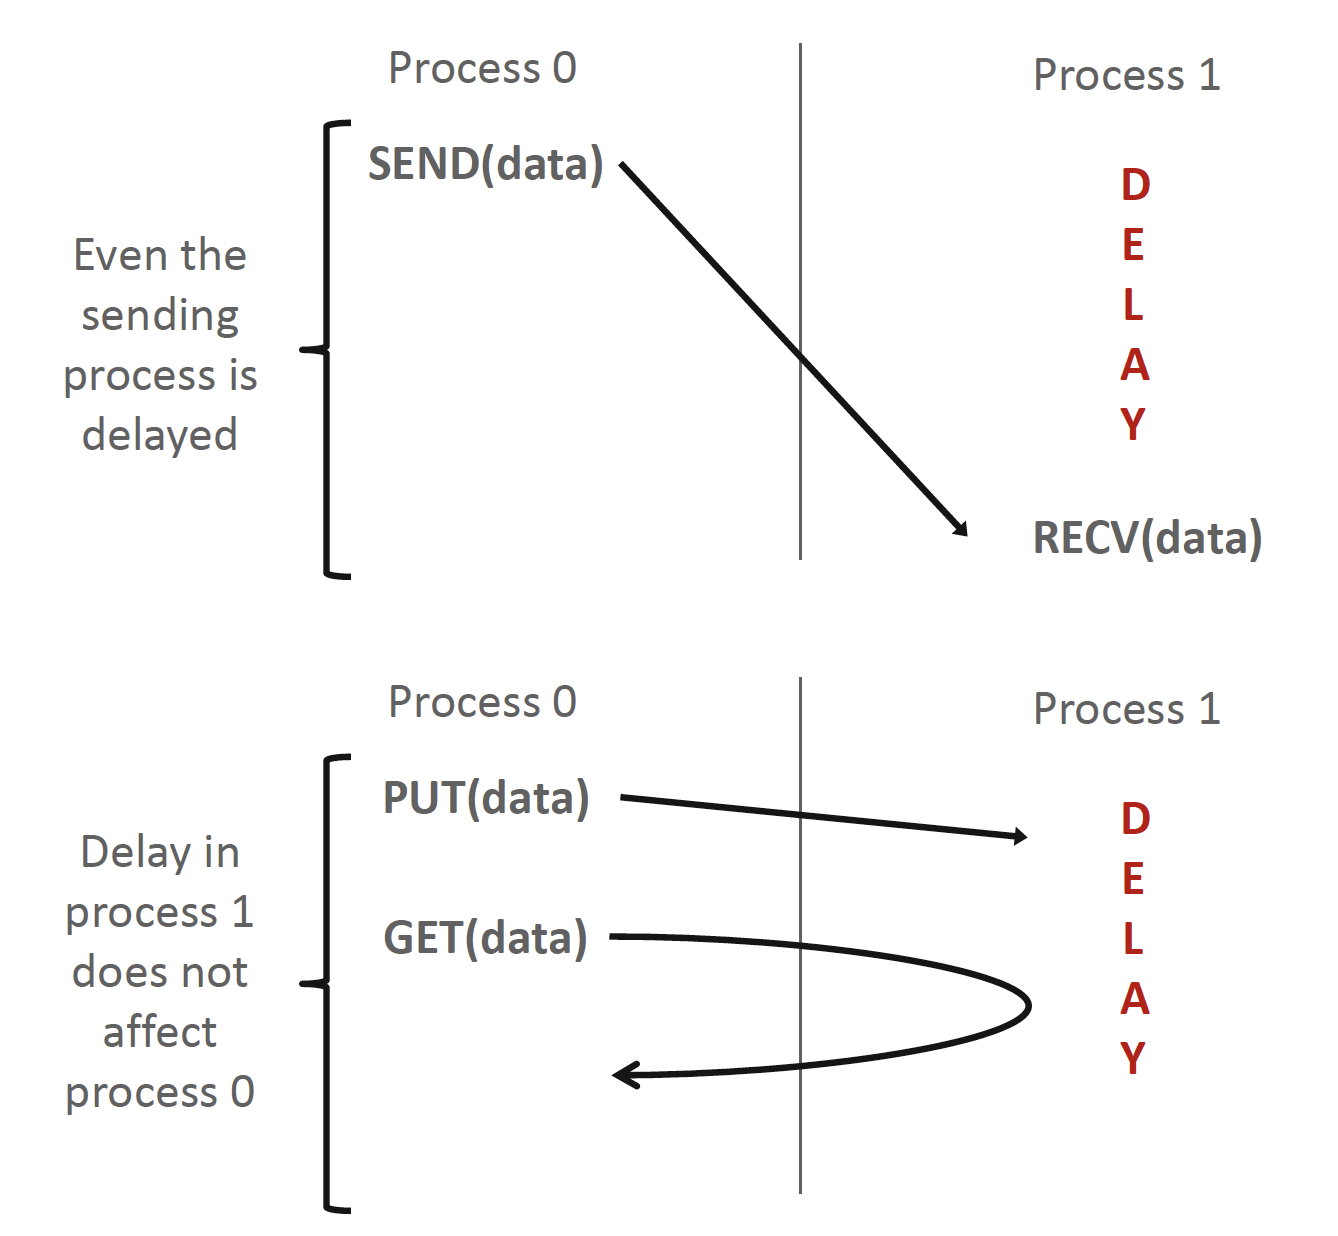
\includegraphics[scale=0.3]{07.MPI_RMA/1sidedvs2sided.png}
    \end{center}
\end{frame}

\begin{frame}[fragile]{Terminology}
\begin{itemize}
\item Origin process: Process with the source buffer, initiates the operation
\item Target process: Process with the destination buffer
\item Epoch: Virtual time where operations are not completed. Data is consistent after new epoch is started.
\item Ordering: order of message between two processes (can be relaxed compared to a strict order)
\end{itemize}

\end{frame}

\begin{frame}[fragile]{One sided communication usage}
Make a memory region remotely accessible: a windows.\\
Creating a window is a collective operation.

Four models exist
\begin{itemize}
    \item \lstinlinePseudo{MPI_WIN_ALLOCATE}: You want to create a buffer and directly make it remotely accessible
    \item \lstinlinePseudo{MPI_WIN_CREATE}: You already have an allocated buffer that you would like to make remotely accessible
    \item \lstinlinePseudo{MPI_WIN_CREATE_DYNAMIC}: You don’t have a buffer yet, but will have one in the future. You may want to dynamically add/remove buffers to/from the window
    \item \lstinlinePseudo{MPI_WIN_ALLOCATE_SHARED}: You want multiple processes on the same node share a buffer
\end{itemize}


%\begin{itemize}
%\item Allocate memory and expose it collectively
%\item Expose collectively already allocated memory
%\item Attach/Dettach memory dynamically to a collectively exposed handler
%\item Communication (put, get, rput, rget)
%\item Accumulate (acc, racc, get\_acc, rget\_acc, fetch\&op, cas)
%\item Synchronization
%\end{itemize}
\end{frame}

\begin{frame}[fragile]{Expose memory}

\begin{Pseudolisting}[]{}
MPI_Win_create(void *ptr, MPI_Aint size, disp_unit,
               MPI_Info info, MPI_Comm comm, MPI_Win win)
MPI_Win_allocate(MPI_Aint size, disp_unit, MPI_Info info,
                 MPI_Comm comm, void *dest_prt, MPI_Win win)
MPI_Win_free(MPI_Win win)
\end{Pseudolisting}
Exposes (and allocate) the memory buffer to other ranks.\\
It is a collective operations among all ranks.\\

\lstinlinePseudo{MPI_Info} contains user configuration.\\
\lstinlinePseudo{MPI_Aint} type that holds any valid address.
\end{frame}

\begin{frame}[fragile]{Dynamic memory}
It is possible to create a window with no memory attached.

\begin{Pseudolisting}[]{}
MPI_Win_create_dynamic(MPI_Info info, MPI_Comm comm,
                       MPI_Win win)
\end{Pseudolisting}

It is possible to attach/detach memory to/from a window.
\begin{Pseudolisting}[]{}
MPI_Win_attach(MPI_Win win, void *ptr, MPI_Aint size)
MPI_Win_detach(MPI_Win win, void *ptr)
\end{Pseudolisting}
\end{frame}

\begin{frame}[fragile]{Data movement}
MPI provides ability to read, write and atomically modify data in remotely accessible memory regions
\begin{itemize}
    \item \lstinlinePseudo{MPI_PUT}
    \item \lstinlinePseudo{MPI_GET}
    \item \lstinlinePseudo{MPI_ACCUMULATE} (atomic)
    \item \lstinlinePseudo{MPI_GET_ACCUMULATE} (atomic)
    \item \lstinlinePseudo{MPI_COMPARE_AND_SWAP} (atomic)
    \item \lstinlinePseudo{MPI_FETCH_AND_OP} (atomic)
\end{itemize}
\end{frame}

\begin{frame}[fragile]{Communication}
Two functions:
Write data into the window (put)
\begin{Pseudolisting}[]{}
MPI_Put(origin_addr, origin_count, origin_datatype, 
        target_rank, target_disp, target_count, target_datatype, win)
\end{Pseudolisting}

Read data from the window (get)
\begin{Pseudolisting}[]{}
MPI_Get(origin_addr, origin_count, origin_datatype, 
        target_rank, target_disp, target_count, 
        target_datatype, win)
\end{Pseudolisting}

\begin{itemize}
\item Non blocking communication
\item Concurrent accesses give undefined behaviour (not an error).
\end{itemize}
\begin{center}
    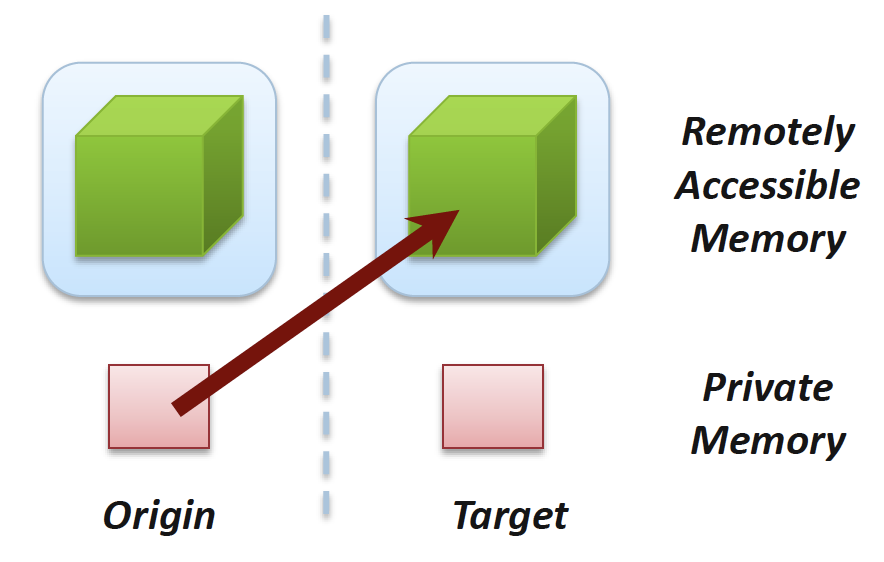
\includegraphics[scale=0.25]{07.MPI_RMA/put.png}\hspace{0.5in}
    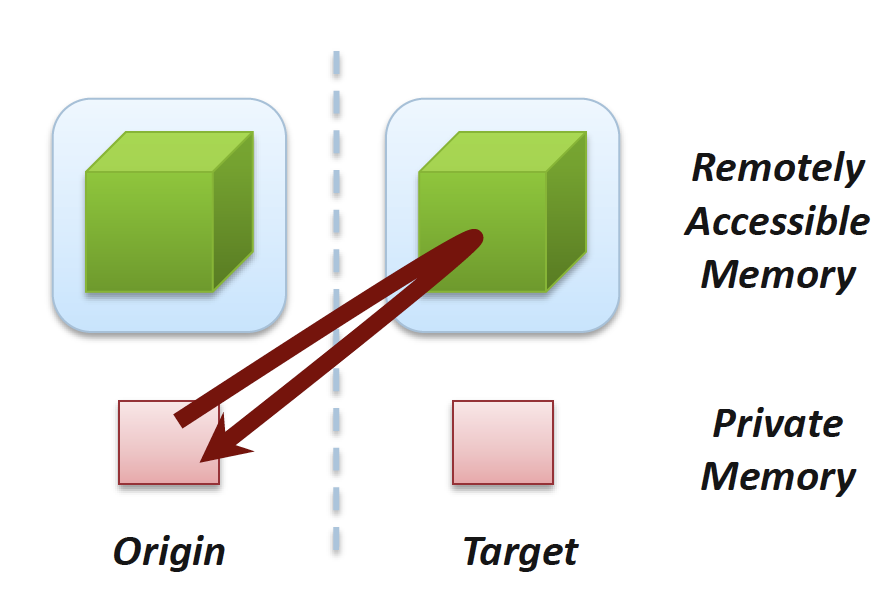
\includegraphics[scale=0.25]{07.MPI_RMA/get.png}
\end{center}
\end{frame}


\begin{frame}[fragile]{Accumulate}
\begin{Pseudolisting}[]{}
MPI_Accumulate(origin_addr, origin_count, origin_datatype,
               target_rank, target_disp, target_count, 
               target_datatype, op, win)
\end{Pseudolisting}

Remote accumulations, replace value in target buffer with accumulated.

\begin{itemize}
\item Only predefined operations
\end{itemize}

Other operations: \lstinlinePseudo{MPI_Fetch_and_op, MPI_Compare_and_swap}
\end{frame}

\begin{frame}[fragile]{Ordering of Operations}
\begin{itemize}
    \item No guaranteed ordering for Put/Get operations
    \item Result of concurrent Puts to the same location is undefined
    \item Result of Get concurrent Put/Accumulate undefined
\item Result of concurrent accumulate operations to the same location are defined according to the order in which the occurred
\end{itemize}
\end{frame}

\begin{frame}[fragile]{Synchronisation}
Three synchronization models provided by MPI:
\begin{itemize}
    \item Fence (active target)
    \item Post-start-complete-wait (generalized active target)
    \item Lock/Unlock (passive target)
\end{itemize}
Data accesses occur within “epochs”
\begin{itemize}
\item Epochs define ordering and completion semantics
\item Synchronization models provide mechanisms for establishing epochs
\end{itemize}
\end{frame}

\begin{frame}[fragile]{Active Target Synchronization}
Collective synchronization model
\begin{Pseudolisting}[]{}
MPI_Win_fence(int assert, MPI_Win win)
\end{Pseudolisting}
\begin{itemize}
    \item Starts andends access and exposure epochs on all processes in the window
    \item All processes in group of “win” do an \lstinlinePseudo{MPI_WIN_FENCE} to open an epoch
    \item Everyone can issue PUT/GET operations to read/write data
    \item Everyone does an \lstinlinePseudo{MPI_WIN_FENCE} to close the epoch
    \item All operations complete at the second fence synchronization
\end{itemize}
\end{frame}


\begin{frame}[fragile]{Passive Target Synchronization}
\begin{Pseudolisting}[]{}
MPI_Win_lock(int locktype, int rank, int assert, MPI_Win win)
MPI_Win_unlock(int rank, MPI_Win win)
MPI_Win_flush(int rank, MPI_Win win)
\end{Pseudolisting}
\begin{itemize}
    \item Lock/Unlock: Begin/end passive mode epoch
    \begin{itemize}
        \item Target process does not make a corresponding MPI call
        \item Can initiate multiple passive target epochs to different processes
        \item Concurrent epochs to same process not allowed (affects threads)
    \end{itemize}
\item Lock type
    \begin{itemize}
    \item SHARED: Other processes using shared can access concurrently
    \item EXCLUSIVE: No other processes can access concurrently
    \end{itemize}
\item Flush: Remotely complete RMA operations to the target process
    \begin{itemize}
    \item After completion, data can be read by target process or a different process
    \end{itemize}
\end{itemize}
%\begin{center}
%    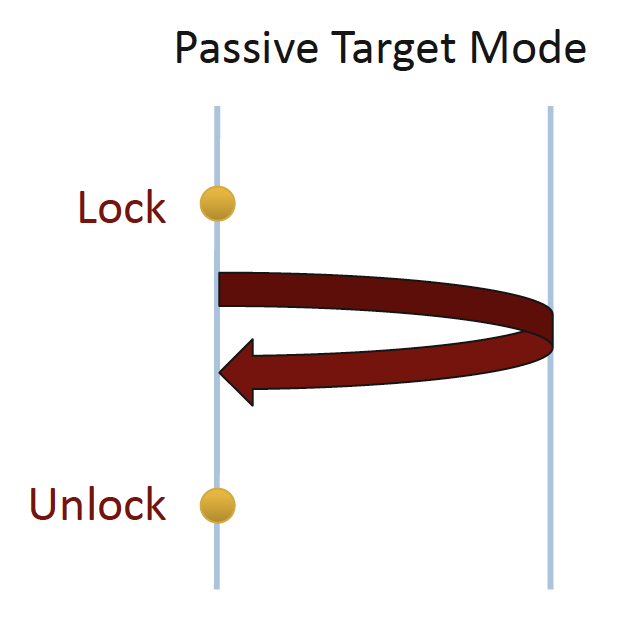
\includegraphics[scale=0.15]{lock.png}
%\end{center}
\end{frame}


\begin{frame}{Practicals}
    \begin{brown2block}{Exercise: 07.MPI\_RMA}
    \begin{enumerate}
        \item \lstinlinePseudo{MPI_Get} + \lstinlinePseudo{MPI_Win_allocate} + \lstinlinePseudo{MPI_Win_fence}
        \item \lstinlinePseudo{MPI_Put} + \lstinlinePseudo{MPI_Win_create} + Passive synchronisation
    \end{enumerate}
        Use a large number of ranks.
    \end{brown2block}
\end{frame}



% THANK YOU SLIDE
\cscsthankyou{Thank you for your attention.}

\end{document}
